%% abtex2-modelo-trabalho-academico.tex, v-1.9.2 laurocesar
%% Copyright 2012-2014 by abnTeX2 group at http://abntex2.googlecode.com/ 
%%
%% This work may be distributed and/or modified under the
%% conditions of the LaTeX Project Public License, either version 1.3
%% of this license or (at your option) any later version.
%% The latest version of this license is in
%%   http://www.latex-project.org/lppl.txt
%% and version 1.3 or later is part of all distributions of LaTeX
%% version 2005/12/01 or later.
%%
%% This work has the LPPL maintenance status `maintained'.
%% 
%% The Current Maintainer of this work is the abnTeX2 team, led
%% by Lauro César Araujo. Further information are available on 
%% http://abntex2.googlecode.com/
%%
%% This work consists of the files abntex2-modelo-trabalho-academico.tex,
%% abntex2-modelo-include-comandos and abntex2-modelo-references.bib
%%

% ------------------------------------------------------------------------
% ------------------------------------------------------------------------
% abnTeX2: Modelo de Trabalho Academico (tese de doutorado, dissertacao de
% mestrado e trabalhos monograficos em geral) em conformidade com 
% ABNT NBR 14724:2011: Informacao e documentacao - Trabalhos academicos -
% Apresentacao
% ------------------------------------------------------------------------
% ------------------------------------------------------------------------

\documentclass[
	% -- opções da classe memoir --
	12pt,				% tamanho da fonte
	openright,			% capítulos começam em pág ímpar (insere página vazia caso preciso)
	oneside,			% para impressão em verso e anverso. Oposto a oneside
	a4paper,			% tamanho do papel. 
	% -- opções da classe abntex2 --
	%chapter=TITLE,		% títulos de capítulos convertidos em letras maiúsculas
	%section=TITLE,		% títulos de seções convertidos em letras maiúsculas
	%subsection=TITLE,	% títulos de subseções convertidos em letras maiúsculas
	%subsubsection=TITLE,% títulos de subsubseções convertidos em letras maiúsculas
	% -- opções do pacote babel --
	english,			% idioma adicional para hifenização
	french,				% idioma adicional para hifenização
	spanish,			% idioma adicional para hifenização
	brazil				% o último idioma é o principal do documento
	]{abntex2}

% ---
% Pacotes básicos 
% ---
\usepackage{lmodern}			% Usa a fonte Latin Modern			
\usepackage[T1]{fontenc}		% Selecao de codigos de fonte.
\usepackage[utf8]{inputenc}		% Codificacao do documento (conversão automática dos acentos)
\usepackage{lastpage}			% Usado pela Ficha catalográfica
\usepackage{indentfirst}		% Indenta o primeiro parágrafo de cada seção.
\usepackage{color}				% Controle das cores
\usepackage{graphicx}			% Inclusão de gráficos
\usepackage[table,xcdraw]{xcolor}

% Please add the following required packages to your document preamble:
% If you use beamer only pass "xcolor=table" option, i.e. 
%\documentclass[xcolor=table]{beamer}
\graphicspath{ {images/} }
\usepackage{microtype} 			% para melhorias de justificação
% ---
		
% ---
% Pacotes adicionais, usados apenas no âmbito do Modelo Canônico do abnteX2
% ---
\usepackage{lipsum}				% para geração de dummy text
\usepackage{multirow}
\usepackage{array}
\usepackage{caption}
\usepackage{float}
\usepackage{pythonhighlight}
\usepackage{listings}
\usepackage{xcolor}
\usepackage{caption}
\usepackage{subcaption}
\colorlet{mygray}{black!30}
\colorlet{mygreen}{green!60!blue}
\colorlet{mymauve}{red!60!blue}

\lstdefinestyle{mystyle}{
    backgroundcolor=\color{white},   
    basicstyle=\ttfamily\footnotesize,
    breakatwhitespace=false,         
    breaklines=true,                 
    captionpos=b,                    
    keepspaces=true,                 
    numbers=left,                    
    numbersep=5pt,                  
    showspaces=false,                
    showstringspaces=false,
    showtabs=false,                  
    tabsize=2,
	texcl=true
}

\lstset{
  backgroundcolor=\color{gray!10},  
  basicstyle=\ttfamily,
  columns=fullflexible,
  breakatwhitespace=false,      
  breaklines=true,                
  captionpos=b,                    
  commentstyle=\color{mygreen}, 
  extendedchars=true,              
  frame=single,                   
  keepspaces=true,             
  keywordstyle=\color{blue},      
  numbers=none,                
  numbersep=5pt,                   
  numberstyle=\tiny\color{blue}, 
  rulecolor=\color{mygray},        
  showspaces=false,               
  showtabs=false,                 
  stepnumber=5,                  
  stringstyle=\color{mymauve},    
  tabsize=3,                      
  title=\lstname,
  showstringspaces=false                
}
\newcolumntype{P}[1]{>{\centering\arraybackslash}p{#1}}

% ---

% ---
% Pacotes de citações
% ---
\usepackage[brazilian,hyperpageref]{backref}	 % Paginas com as citações na bibl
\usepackage[alf]{abntex2cite}	% Citações padrão ABNT

% --- 
% CONFIGURAÇÕES DE PACOTES
% --- 

% ---
% Configurações do pacote backref
% Usado sem a opção hyperpageref de backref
\renewcommand{\backrefpagesname}{Citado na(s) página(s):~}
% Texto padrão antes do número das páginas
\renewcommand{\backref}{}
% Define os textos da citação
\renewcommand*{\backrefalt}[4]{
	\ifcase #1 %
		Nenhuma citação no texto.%
	\or
		Citado na página #2.%
	\else
		Citado #1 vezes nas páginas #2.%
	\fi}%
% ---

% ---
% Informações de dados para CAPA e FOLHA DE ROSTO
% ---
\titulo{Relatório}
\autor{Gabriel Medeiros Lopes Carneiro\\
       Paulo Arthur Sens Coelho\\
       Erik Kazuo Sugawara}
\local{Florianópolis, SC}
\data{2022}
\orientador{Odorico Machado Mendizabal}
\instituicao{%
  Universidade Federal de Santa Catarina
  \par
  Departamento de Informática e Estatística
  \par
  Programa de Graduação}
\tipotrabalho{Relatório (Graduação)}
% O preambulo deve conter o tipo do trabalho, o objetivo, 
% o nome da instituição e a área de concentração 
\preambulo{Trabalho apresentado para avaliação de uma implementação
de uma biblioteca para comunicação confiável e algoritmo distribuído,
na disciplina INE 5418 - Computação Distribuída, sob Orientação do
Prof. Dr. Odorico Machado Mendizabal}
% ---


% ---
% Configurações de aparência do PDF final

% alterando o aspecto da cor azul
\definecolor{blue}{RGB}{41,5,195}

% informações do PDF
\makeatletter
\hypersetup{
     	%pagebackref=true,
		pdftitle={\@title}, 
		pdfauthor={\@author},
    	pdfsubject={\imprimirpreambulo},
	    pdfcreator={LaTeX with abnTeX2},
		pdfkeywords={abnt}{latex}{abntex}{abntex2}{trabalho acadêmico}, 
		colorlinks=true,       		% false: boxed links; true: colored links
    	linkcolor=blue,          	% color of internal links
    	citecolor=blue,        		% color of links to bibliography
    	filecolor=magenta,      		% color of file links
		urlcolor=blue,
		bookmarksdepth=4
}
\makeatother
% --- 

% --- 
% Espaçamentos entre linhas e parágrafos 
% --- 

% O tamanho do parágrafo é dado por:
\setlength{\parindent}{1.3cm}

% Controle do espaçamento entre um parágrafo e outro:
\setlength{\parskip}{0.2cm}  % tente também \onelineskip

% ---
% compila o indice
% ---
\makeindex
% ---

% ----
% Início do documento
% ----
\begin{document}

% Retira espaço extra obsoleto entre as frases.
\frenchspacing

% ----------------------------------------------------------
% ELEMENTOS PRÉ-TEXTUAIS
% ----------------------------------------------------------
% \pretextual

% ---
% Capa
% ---
\imprimircapa
% ---

% ---
% Folha de rosto
% (o * indica que haverá a ficha bibliográfica)
% ---
\imprimirfolhaderosto*
% ---

% ---
% Inserir a ficha bibliografica
% ---

% Isto é um exemplo de Ficha Catalográfica, ou ``Dados internacionais de
% catalogação-na-publicação''. Você pode utilizar este modelo como referência. 
% Porém, provavelmente a biblioteca da sua universidade lhe fornecerá um PDF
% com a ficha catalográfica definitiva após a defesa do trabalho. Quando estiver
% com o documento, salve-o como PDF no diretório do seu projeto e substitua todo
% o conteúdo de implementação deste arquivo pelo comando abaixo:
%
% \begin{fichacatalografica}
%     \includepdf{fig_ficha_catalografica.pdf}
% \end{fichacatalografica}
\begin{fichacatalografica}
	\vspace*{\fill}					% Posição vertical
	\hrule							% Linha horizontal
	\begin{center}					% Minipage Centralizado
		\begin{minipage}[c]{12.5cm}		% Largura

			\imprimirautor

			\hspace{0.5cm} \imprimirtitulo  / \imprimirautor. --
			\imprimirlocal, \imprimirdata-

			\hspace{0.5cm} \pageref{LastPage} p. : il. (algumas color.) ; 30 cm.\\

			\hspace{0.5cm} \imprimirorientadorRotulo~\imprimirorientador\\

			\hspace{0.5cm}
			\parbox[t]{\textwidth}{\imprimirtipotrabalho~--~\imprimirinstituicao,
				\imprimirdata.}\\

			\hspace{0.5cm}
			1. Computação Distribuída.
			2. Sockets.
			3. Ordem Causal.
			4. Ordem Total.
			5. Biblioteca.\\

			\hspace{8.75cm} CDU 02:141:005.7\\

		\end{minipage}
	\end{center}
	\hrule
\end{fichacatalografica}
%
% ---

% ---
% Inserir folha de aprovação
% ---

% Isto é um exemplo de Folha de aprovação, elemento obrigatório da NBR
% 14724/2011 (seção 4.2.1.3). Você pode utilizar este modelo até a aprovação
% do trabalho. Após isso, substitua todo o conteúdo deste arquivo por uma
% imagem da página assinada pela banca com o comando abaixo:
%
% \includepdf{folhadeaprovacao_final.pdf}
%
\begin{folhadeaprovacao}

	\begin{center}
		{\ABNTEXchapterfont\large\imprimirautor}

		\vspace*{\fill}\vspace*{\fill}
		\begin{center}
			\ABNTEXchapterfont\bfseries\Large\imprimirtitulo
		\end{center}
		\vspace*{\fill}

		\hspace{.45\textwidth}
		\begin{minipage}{.5\textwidth}
			\imprimirpreambulo
		\end{minipage}%
		\vspace*{\fill}
	\end{center}


	\assinatura{\textbf{\imprimirorientador} \\ Orientador}

	\begin{center}
		\vspace*{0.5cm}
		{\large\imprimirlocal}
		\par
		{\large\imprimirdata}
		\vspace*{1cm}
	\end{center}

\end{folhadeaprovacao}
% ---
% RESUMOS
% ---

% resumo em português



% ---

% ---
% inserir lista de ilustrações
% ---
\pdfbookmark[0]{\listfigurename}{lof}
\listoffigures*
\cleardoublepage
% ---

% ---
% inserir lista de tabelas
% ---

% ---

% ---
% inserir lista de abreviaturas e siglas
% ---

% ---

% ---
% inserir lista de símbolos
% ---

% ---
% inserir o sumario
% ---
\pdfbookmark[0]{\contentsname}{toc}
\tableofcontents*
\cleardoublepage
% ---



% ----------------------------------------------------------
% ELEMENTOS TEXTUAIS
% ----------------------------------------------------------
\textual

% ----------------------------------------------------------
% Introdução (exemplo de capítulo sem numeração, mas presente no Sumário)
% ----------------------------------------------------------
\chapter*[Introdução]{Identificação}
\addcontentsline{toc}{chapter}{Identificação}
% ----------------------------------------------------------

\begin{center}
	Universidade Federal de Santa Catarina \\
	Departamento de Informática e Estatística\\
	Ciências da Computação \\
	INE 5425 - Modelagem e Simulação \\
	\vspace*{5cm}
	\textbf{Contato} \\
	\vspace*{1cm}
    Gabriel Medeiros Lopes Carneiro\\
	Email: gabriel.mlc@grad.ufsc.br\\
	\vspace*{0.5cm}
    Paulo Arthur Sens Coelho\\
	Email: paulo.sens.coelho@grad.ufsc.br\\
	\vspace*{0.5cm}
	Erik Kazuo Sugawara \\
	Email: erik.sugawara@grad.ufsc.br \\
\end{center}
% ----------------------------------------------------------
% PARTE
% ----------------------------------------------------------
\part{Biblioteca de Comunicação Confiável}
% ----------------------------------------------------------

% ---
% Capitulo com exemplos de comandos inseridos de arquivo externo 
% ---
\include{abntex2-modelo-include-comandos}
% ---

% ---
% Capitulo de revisão de literatura
% ---
\chapter{Sobre o Trabalho}

\section{Introdução}
Um sistema distribuído é caracterizado por componentes localizados em uma rede de computadores,
que se comunicam e coordenam suas ações através de troca de mensagens e que podem sofrer
influências internas ou externas, as quais podem prejudicar a sua interoperabilidade. Através da
concorrência entre os componentes comunicantes, o estado de seus dados se tornam inconsistentes a medida que não existe uma sincronização.
Seja por conta da ausência de um relógio global ou de uma memória compartilhada, se torna impossível realizar uma sincronização perfeita
entre as trocas de mensagens. Além disso, em seu aspecto físico, componentes são suscetíveis a falha
e podem impedir o funcionamento do sistema. Sendo assim, o objetivo deste trabalho é criar uma
biblioteca de comunicação confiável que seja capaz de garantir a ordem no recebimento e envio
de mensagens seguindo critérios de ordem causal e total, de modo que os participantes
da comunicação consigam estabelecer troca de mensagens do tipo 1 : 1 e 1 : n. 

\section{Metodologia}
Para realizar a criação da biblioteca foi escolhida a linguagem Python por sua versatilidade
e legibilidade. Em conjunto, foi usado a biblioteca de Multiprocessos para permitir que os processos
que instanciam os sockets sejam possíveis de serem executados em paralelo,
garantindo o recebimento e envio de mensagens de múltiplos nodos.
Cada nodo contém dois processos que instanciam sockets: o primeiro é utilizado para o recebimento de mensagens
e o segundo é utilizado para enviar mensagens, uma vez que não conseguimos reutilizar o mesmo socket para realizar
operações de envio e recebimento. Para garantir a entrega dos dados, foi utilizado o Protocolo TCP.  
No socket foi utilizado o domínio AF\_INET para criarmos um socket capaz utilizar os endereços com seus respectivos Ip e Porta,
dessa forma os nodos são capazes de comunicar entre si. Além disso,
a garantia do recebimento de pacotes ponto a ponto facilita a elaboração de uma biblioteca
mais robusta.

\chapter{Desenvolvimento}
\section{Biblioteca}
\subsection{Nodo}

A estrutura de cada nodo é composta por três tipos de buffer: do processo, de entrada e de saída.
O de processo é responsável por armazenar as mensagens que precisam aguardar outras chegarem.
O buffer de entrada armazena os IDs de cada mensagens e verifica se a mensagem já pode ser entregue.
O buffer de saída adiciona os IDs em cada mensagem para cada um dos endereços de nodo.
Para comunicação são utilizados dois sockets: um para recebimento de
mensagens e outro para envios. Cada socket tem o seu próprio endereço,
dessa forma um nodo tem dois sockets com diferentes portas. Na figura \ref{fig:nodo},
podemos ver o esquema de um nodo.

\begin{figure}[!h]
    \centering
    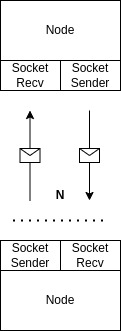
\includegraphics[scale=0.9]{node.jpg}
    \caption{Estrutura de um nodo}
    \label{fig:nodo}
\end{figure}

\section{Mensagem}
Internamente as mensagens são compostas por quatro atributos: dados a serem enviados, id da mensagem,
id do processo e endereço do processo. Cada mensagem é transferido na forma de bytes,
onde é realizado um parse dela. Em nossa biblioteca, enviamos uma string com o seguinte
corpo: DataTxt \# MsgID \# ProcessID \# ProcessAddress.

\subsection{Recebimento de mensagens}
O método responsável por receber as mensagens verifica se a mensagem recebida
está no buffer do processo. Se sim, ignora a mensagem. Do contrário, verifica se
ela está no buffer de entrada e se já pode ser entregue. Se a mensagem está em seu estado válido,
então a mensagem é entregue.

\begin{figure}[!h]
    \centering
    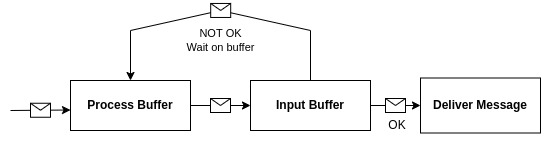
\includegraphics[scale=0.8]{recv.jpg}
    \caption{Estrutura do recebimento de mensagens}
    \label{fig:recv}
\end{figure}

\subsection{Envio de mensagens}
Para enviar as mensagens é necessário adicionar o ID em cada uma delas antes do envio.
Sendo assim, foi utilizado um buffer de saída que armazena os IDs de cada mensagem para cada um dos
comunicantes.
\begin{figure}[!h]
    \centering
    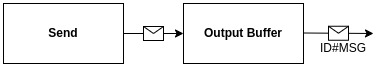
\includegraphics[scale=0.8]{send.jpg}
    \caption{Estrutura do envio de mensagens}
    \label{fig:send}
\end{figure}

\section{Algoritmo Token Ring}
Nesse algoritmo é construído um anel lógico com os processos comunicantes.
Em sua inicialização o processo 0 recebe um token. Ele deve circular 
pelo anel passando de um processo k para o k + 1. Quando o processo
recebe o token ele pode executar a região crítica (uma única vez) e, após sair,
passa o token para o próximo processo. Se o processo não desejar entrar na 
região crítica, deve apenas passar o token para o próximo processo.

\section{Execução}
\section{Resultados}
Para verificar o funcionamento das mensagens, realizamos um teste onde o nodo 1 envia
duas mensagens para o nodo 2. Na figura \ref{fig:confirmado}, é mostrado a saída
indicando que a mensagem foi entregue corretamente.

\begin{figure}[!h]
    \centering
    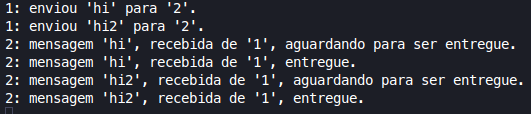
\includegraphics[scale=0.9]{confirmado.png}
    \caption{Envio de mensagens sendo entregue entre os processos.}
    \label{fig:confirmado}
\end{figure}


\section{Conclusão}
\section{Referências}
%\section{Conclusões e/ou Recomendações}
%\section{Referências}

% ----------------------------------------------------------
% Finaliza a parte no bookmark do PDF
% para que se inicie o bookmark na raiz
% e adiciona espaço de parte no Sumário
% ----------------------------------------------------------
\phantompart

% ---
% Conclusão (outro exemplo de capítulo sem numeração e presente no sumário)
% ---
%\chapter*[Conclusão]{Conclusão}
%\addcontentsline{toc}{chapter}{Conclusão}
% ---

%\chapter{Referências Bibliográfica}

%BARBETTA, Pedro A.; REIS, Marcelo M. e BORNIA, Antonio C. Estatística para cursos de
%Engenharia e Informática. São Paulo: Editora Atlas S.A., 2010


% ----------------------------------------------------------
% ELEMENTOS PÓS-TEXTUAIS
% ----------------------------------------------------------
\postextual
% ----------------------------------------------------------

% ----------------------------------------------------------
% Referências bibliográficas
% ----------------------------------------------------------
\bibliography{abntex2-modelo-references}
% ----------------------------------------------------------
% Glossário
% ----------------------------------------------------------
%
% Consulte o manual da classe abntex2 para orientações sobre o glossário.
%
%\glossary

\begin{anexosenv}
\chapter{Biblioteca}
\section{Código}

\chapter{Algoritmo}
\end{anexosenv}
%---------------------------------------------------------------------
% INDICE REMISSIVO
%---------------------------------------------------------------------
\phantompart
\printindex
%---------------------------------------------------------------------

\end{document}